\newpage
\section{Escalonamento}\label{sec:Escalonamento}

O escalonador é um subsistema do SO encarregado de direcionar a prioridade de entrada dos processos na \emph{CPU} os algoritmos avaliam o cenário disposto pelo sistema e com isso determina a lógica empregada para resolver qual processo será processado é importante lembrar que algumas variáveis necessitam de mais processo estes ocuparão a \emph{CPU} por um tempo maior e não precisam da intervenção do usuário. Os processos que precisam de mais entradas e saídas de dados, ou seja, o processo demanda intervenção do usuário \cite{Tanenbaum2016}.
\begin{figure}[htpb]
    \centering
   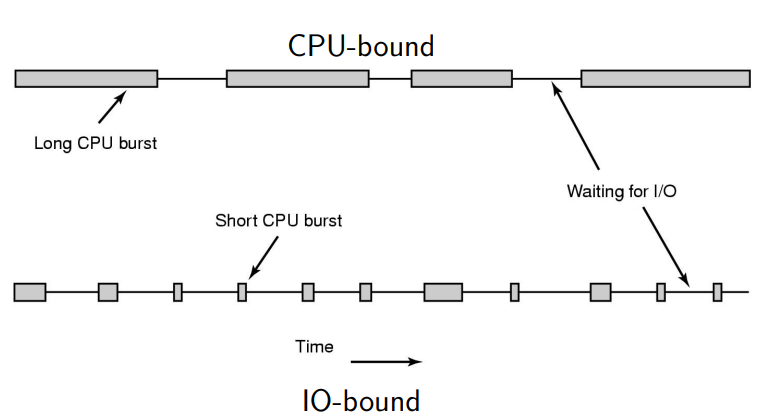
\includegraphics[scale=.4]{imagens/escalonamento1.png}
   \caption{Comportamento de processos. \cite{Tanenbaum2016}}
   \label{fig:escalonador}
\end{figure}

\subsection{Categorias de algoritimo de escalonamento}

Diferentes algoritmos de escalonamento são implementados para tratar condição que acontece nas diferentes áreas de aplicação do SO principalmente processos identificados para objetivos diferentes. Cada sistema tem particularidades que devem ser levadas em consideração pelo escalonador \cite{Tanenbaum2016}.\\
\\É necessário distinguir três ambientes:
    \begin{enumerate}
        \item Lote
        \item Interativo
        \item Tempo real 
    \end{enumerate}


Sistema em lote são bastante comuns por sua otimização no tempo de retorno e maximiza o número de horas de trabalho e muitas vezes aplicáveis a outras situações também, o que torna seu estudo interessante, mesmo para pessoas não envolvidas na computação corporativa de grande porte \cite{Tanenbaum2016}.\\
Sistemas interativos tem objetivo de otimizar o tempo de resposta, mesmo que nenhum processo execute de modo intencional para sempre, um erro em um programa pode levar um processo a impedir indefinidamente que todos os outros executem. Os servidores \emph{Linux} também caem nessa categoria, visto que eles normalmente servem a múltiplos usuários (remotos), todos os quais estão muito apressados, assim como usuários de computadores \cite{Tanenbaum2016}.\\
Em sistemas de tempo real, os processos sabem que eles não podem executar por longos períodos e em geral realizam o seu trabalho e bloqueiam rapidamente. A diferença com os sistemas interativos é que os de tempo real executam apenas programas que visam ao progresso da aplicação à mão \cite{Tanenbaum2016}.